
% This LaTeX was auto-generated from MATLAB code.
% To make changes, update the MATLAB code and republish this document.

\documentclass{article}
\usepackage{graphicx}
\usepackage{color}

\sloppy
\definecolor{lightgray}{gray}{0.5}
\setlength{\parindent}{0pt}

\begin{document}

    
    
\subsection*{Contents}

\begin{itemize}
\setlength{\itemsep}{-1ex}
   \item Analyze Sensordata
   \item Rearrange data
   \item Plots
   \item accelerometer, gyro, orientation, motor commands
   \item Altitude
   \item motorcommands
   \item 2D Position \& Velocity
   \item Velocity, Optical Flow
\end{itemize}


\subsection*{Analyze Sensordata}

\begin{par}
=============================== AUTHOR Fabian Riether CREATE DATE 2015/08/25 PURPOSE This scripts plots tons of data from a flight data saved to a RSdata.mat-file onboard the drone. Additionaly, it rearranges data to be used in the SoftwareinTheLoop\_Compensator simulink model SPECIAL NOTES ===============================  2015/08/25 created ==================================
\end{par} \vspace{1em}
\begin{verbatim}
clear
close all
clc
load bestestsquared
\end{verbatim}


\subsection*{Rearrange data}

\begin{verbatim}
%Load all parameters
parameters_estimationcontrol;

%Choose which data to plot
if ( exist('rt_yout','var') && exist('rt_yout_sim','var') )
    [s,v] = listdlg('PromptString','Select data to plot:',...
                'SelectionMode','single',...
                'ListString',{'recorded','simulated'});
    if (v==0)
        disp('No selection made, plotting recorded data');
    else
      if (s==1)
        results = rt_yout;
      else
        results = rt_yout_sim;
      end;
    end;

elseif exist('rt_yout','var')
    results = rt_yout;
elseif exist('rt_yout_sim','var')
    results = rt_yout_sim;
else
    disp('No data to plot');
    return;
end;

%Aug31rst+ recordings file version
if ( size(results.signals,2)>24)
    RSrun_motorcommands = [results.time results.signals(1).values];
    RSrun_controlMode   = [results.time,results.signals(14).values];
    RSrun_orient_ref     = [results.time,results.signals(15).values(:,4:6)];
    RSrun_pos_ref       = [results.time,results.signals(15).values(:,1:3)];
    RSrun_sensordata    = [results.time results.signals(16).values results.signals(17).values results.signals(18).values results.signals(19).values results.signals(20).values permute(results.signals(21).values,[ 1 2 3]) permute(results.signals(22).values,[1 2 3]) results.signals(23).values ];
    RSrun_opticalFlow   = [results.time,results.signals(24).values];
    RSrun_sensordataCalib  = [results.signals(25).values(1,:)];
    RSrun_posVIS        = [results.time,results.signals(26).values];
    RSrun_usePosVIS     = [results.time,results.signals(27).values];

    RSrun_states_estim  = results.time;
    for i=2:13
        RSrun_states_estim = [RSrun_states_estim results.signals(i).values];
    end;

    if (size(results.signals,2)>27)
        RSrun_batteryStatus = [results.time,results.signals(28).values];
    end;

%takeoff flag added!
if ( size(results.signals,2)>28)
    RSrun_takeoff_flag = [results.time,results.signals(29).values];
end;

%--old recordings-file-version
elseif (size(results.signals(2).values,2)==1)

    RSrun_sensordata    = [results.time results.signals(2).values results.signals(3).values results.signals(4).values results.signals(5).values results.signals(6).values permute(results.signals(7).values,[ 1 2 3]) permute(results.signals(8).values,[1 2 3]) results.signals(9).values ];
    RSrun_orient_ref    = [results.time,results.signals(22).values(:,4:6)];
    RSrun_pos_ref       = [results.time,results.signals(22).values(:,1:3)];
    RSrun_controlMode   = [results.time,((RSrun_pos_ref(:,1)~=0) & (RSrun_pos_ref(:,2)~=0))];
    RSrun_motorcommands = [results.time results.signals(1).values];
    RSrun_opticalFlow = [results.time,results.signals(23).values];
    RSrun_posVIS        = [results.time,results.signals(24).values];

    RSrun_states_estim  = results.time;

    for i=10:21
        RSrun_states_estim = [RSrun_states_estim results.signals(i).values];
    end;

%--Aug 14-Aug 31rst recordings-file-version
else

    RSrun_sensordata    = [results.time results.signals(3).values results.signals(4).values results.signals(5).values results.signals(6).values results.signals(7).values permute(results.signals(8).values,[ 1 2 3]) permute(results.signals(9).values,[1 2 3]) results.signals(10).values ];
    RSrun_motorcommands = [results.time results.signals(1).values];
    RSrun_opticalFlow   = [results.time,results.signals(23).values];
    RSrun_posVIS        = [results.time,results.signals(24).values];
    RSrun_orient_ref    = [results.time,results.signals(2).values(:,4:6)];
    RSrun_pos_ref       = [results.time,results.signals(2).values(:,1:3)];
    RSrun_controlMode   = [results.time,((RSrun_pos_ref(:,1)~=0) & (RSrun_pos_ref(:,2)~=0))];

    RSrun_states_estim  = results.time;
    for i=11:22
        RSrun_states_estim = [RSrun_states_estim results.signals(i).values];
    end;
end;
\end{verbatim}


\subsection*{Plots}

\begin{verbatim}
%%-------------
\end{verbatim}


\subsection*{accelerometer, gyro, orientation, motor commands}

\begin{verbatim}
visUpdatesAvlble = (RSrun_posVIS(:,2)~=-99);

%figure('Name','Sensors, Orientation & Motors','Position',[100 100 600 700]);

%accelerometer
%h(1)=subplot(4,1,1);
figure

plot(RSrun_sensordata(:,1),RSrun_sensordata(:,2:4))
title('Acceleration')
ylabel({'IMUaccel $[m/s^2]$'},'Interpreter','latex');
legend({'$\tilde{a}_x$' '$\tilde{a}_y$' '$\tilde{a}_z$'},'Interpreter','latex','Location','best');
%ylim([-12 12])


%gyro
%h(2)=subplot(4,1,2);
figure
plot(RSrun_sensordata(:,1),RSrun_sensordata(:,5:end-2))
title('Gyro')
ylabel({'IMUgyro $[rad/s]$'},'Interpreter','latex');
legend({ '$w_x$' '$w_y$' '$w_z$'},'Interpreter','latex','Location','best');
%ylim([-1 1])

%state estimates
%h(3)=subplot(4,1,3);
figure
plot(RSrun_states_estim(:,1),RSrun_states_estim(:,5:7),'.-'); hold all;
plot(RSrun_orient_ref(:,1),RSrun_orient_ref(:,2:end));
if (any(visUpdatesAvlble))
    plot(RSrun_posVIS(visUpdatesAvlble,1),RSrun_posVIS(visUpdatesAvlble,5),'o');
    legend({'yaw $\hat{\psi}$' 'pitch $\hat{\theta}$' 'roll $\hat{\phi}$' '$\psi_{d}$' '$\theta_{d}$' '$\phi_{d}$' '$\hat{\psi}_{VIS}$'  },'Interpreter','latex','Location','best');
else
    legend({'yaw' 'pitch' 'roll' 'yaw_{ref}' 'pitch_{ref}' 'roll_{ref}'},'Location','best');
end;
title('Euler Angles')
ylabel({'orientation $[rad]$'},'Interpreter','latex');

%ylim([-0.3 0.3])
\end{verbatim}

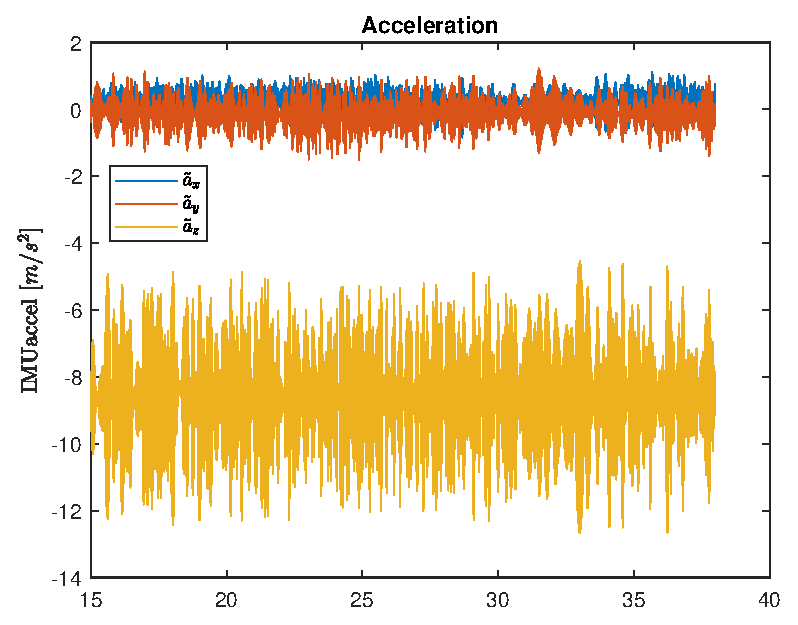
\includegraphics [width=4in]{FlightAnalyzer2_01.eps}

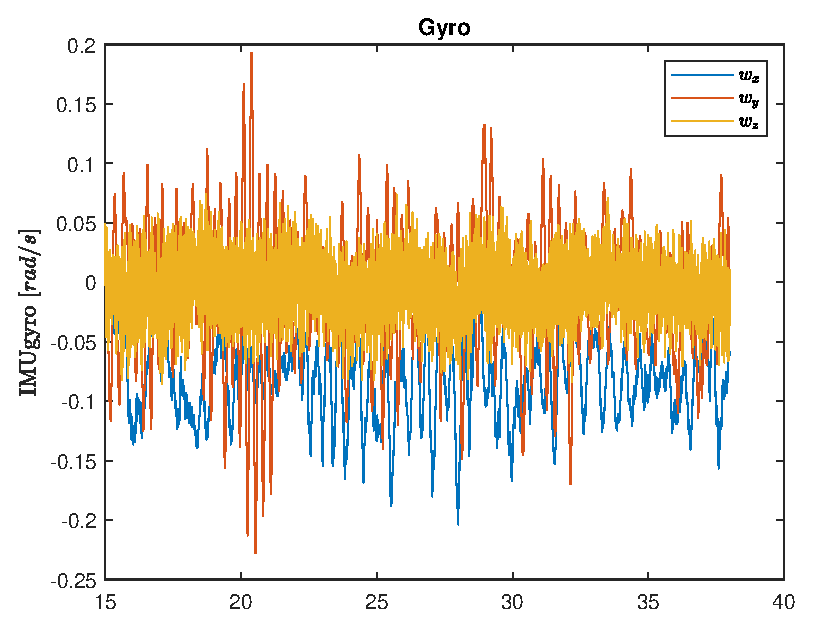
\includegraphics [width=4in]{FlightAnalyzer2_02.eps}

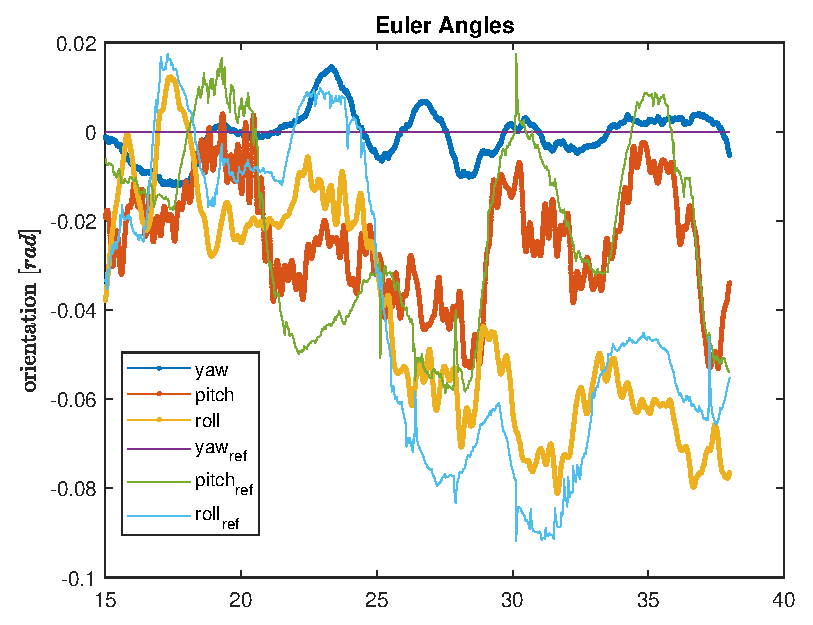
\includegraphics [width=4in]{FlightAnalyzer2_03.eps}


\subsection*{Altitude}

\begin{verbatim}
figure('Name','Altitude');


% altitude from pressure (for comparison only)
altPrs = (RSrun_sensordata(:,9) - RSrun_sensordataCalib(1,7))/(quadEDT.altToPrs_gain);
hold off;
plot(RSrun_sensordata(:,1), altPrs); hold all;
% altitude from sonar
plot(RSrun_sensordata(:,1), -RSrun_sensordata(:,8),'LineWidth',2);

% altitude from KF
plot(RSrun_states_estim(:,1),RSrun_states_estim(:,4),'LineWidth',3);

% altitude reference
plot(RSrun_pos_ref(:,1),RSrun_pos_ref(:,4),'g','LineWidth',2);

% altitude from vision
visUpdatesAvlble = (RSrun_posVIS(:,2)~=-99);
plot(RSrun_posVIS(visUpdatesAvlble,1),-RSrun_posVIS(visUpdatesAvlble,4),'o','LineWidth',3);

legend({'Pressure $\hat{z}_{prs}$'  'Sonar $\hat{z}_{snr}$' 'Kalman-estimate $\hat z$' 'Reference $z_{d}$' 'Vision $\hat{z}_{VIS}$' },'Interpreter','latex','Location','best');
ylim([-3.5 1]);
xlabel({'t[s]'},'Interpreter','latex');
ylabel({'altitude [m]'},'Interpreter','latex');
title('Altitude')
\end{verbatim}

        \color{lightgray} \begin{verbatim}Warning: Ignoring extra legend entries. 
\end{verbatim} \color{black}
    
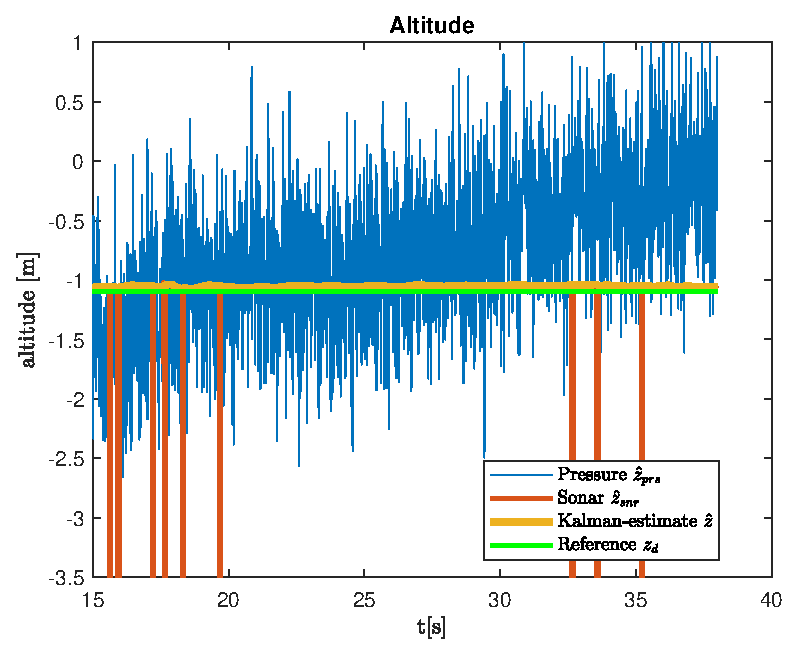
\includegraphics [width=4in]{FlightAnalyzer2_04.eps}


\subsection*{motorcommands}

\begin{verbatim}
figure
plot(RSrun_motorcommands(:,1),RSrun_motorcommands(:,2:end));
ylabel({'motor commands'},'Interpreter','latex');
xlabel({'t [s]'},'Interpreter','latex');
legend({'m$_1$' 'm$_2$' 'm$_3$' 'm$_4$'},'Interpreter','latex');
title('Motor Commands vs. Time')
ylim([-600 600])
\end{verbatim}

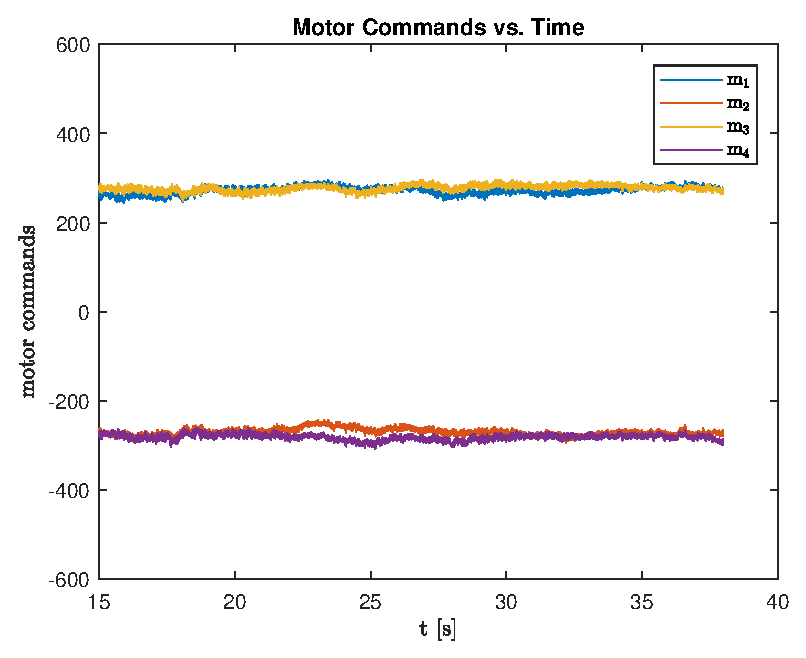
\includegraphics [width=4in]{FlightAnalyzer2_05.eps}


\subsection*{2D Position \& Velocity}

\begin{verbatim}
visUpdatesAvlble = (RSrun_posVIS(:,2)~=-99);

figure%('Name','Positions & Velocities','Position',[100 100 600 700]);
%subplot(6,1,1:2);

%Trajectory
plot(RSrun_states_estim(:,3),RSrun_states_estim(:,2));
hold all;
plot(RSrun_states_estim(1,3),RSrun_states_estim(1,2),'rx');
plot(RSrun_states_estim(end,3),RSrun_states_estim(end,2),'gx');
plot(RSrun_posVIS(visUpdatesAvlble,3),RSrun_posVIS(visUpdatesAvlble,2),'o-');
%set(gca,'xaxisLocation','top')
%set(gca,'Xdir','reverse')
legend({'$\hat{Pos}$','start','finish','$\hat{Pos}_{VIS}$'},'Location','best','Interpreter', 'latex')
%ylim([-.3 .3]);
title('Drone Trajectory')
xlabel({'$X$ [m]'},'Interpreter','latex');
ylabel({'$Y$ [m]'},'Interpreter','latex');
%axis equal

%Positions
figure
axis normal
plot(RSrun_states_estim(:,1),RSrun_states_estim(:,2));hold all;
plot(RSrun_posVIS(visUpdatesAvlble,1),RSrun_posVIS(visUpdatesAvlble,2),'o');
legend({'$\hat{X}$','$\hat{X}_{VIS}$'},'Interpreter','latex')
ylim([-.7 .7])
ylabel({'$X$ [m]'},'Interpreter','latex');

figure
plot(RSrun_states_estim(:,1),RSrun_states_estim(:,3));   hold all;
plot(RSrun_posVIS(visUpdatesAvlble,1),RSrun_posVIS(visUpdatesAvlble,3),'o');
legend({'$\hat{Y}$','$\hat{Y}_{VIS}$'},'Interpreter','latex')
ylim([-.5 .5])
ylabel({'$Y$ [m]'},'Interpreter','latex');

%Velocities
h(3)=subplot(12,1,9:10);
plot(RSrun_opticalFlow(:,1),20*RSrun_opticalFlow(:,2),'.-'); hold all;
plot(RSrun_states_estim(:,1),RSrun_states_estim(:,8));
ylabel('$\dot x$ [m/s]','Interpreter','latex');
legend({'$\dot{x}_{opt. flow}$' '$\hat{\dot x}$'},'Interpreter','latex');

figure
plot(RSrun_opticalFlow(:,1),20*RSrun_opticalFlow(:,3),'.-'); hold all;
plot(RSrun_states_estim(:,1),RSrun_states_estim(:,9));
xlabel({'t [s]'},'Interpreter','latex');
ylabel('$\dot y$ [m/s]','Interpreter','latex');
legend({'$\dot{y}_{opt. flow}$' '$\hat{\dot y}$'},'Interpreter','latex');

%set(h(1:end-1),'xticklabel',[])
linkaxes(h,'x');
\end{verbatim}

        \color{lightgray} \begin{verbatim}Warning: Ignoring extra legend entries. 
Warning: Ignoring extra legend entries. 
Warning: Ignoring extra legend entries. 
Warning: Excluding ColorBars, Legends and non-axes 
\end{verbatim} \color{black}
    
\includegraphics [width=4in]{FlightAnalyzer2_06.eps}

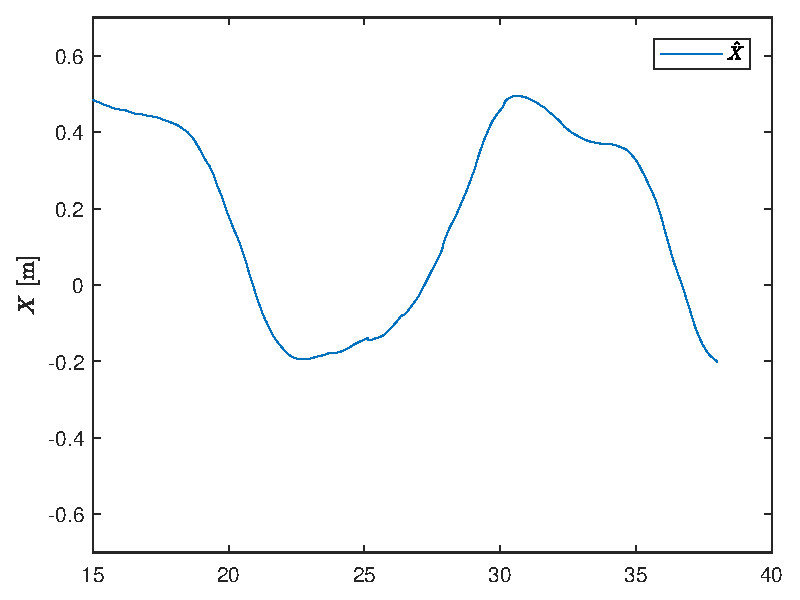
\includegraphics [width=4in]{FlightAnalyzer2_07.eps}

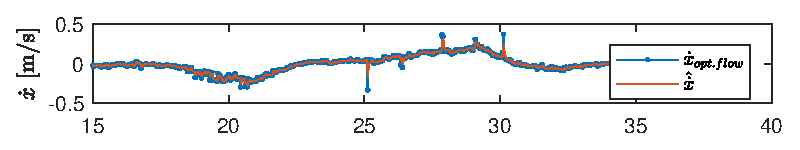
\includegraphics [width=4in]{FlightAnalyzer2_08.eps}

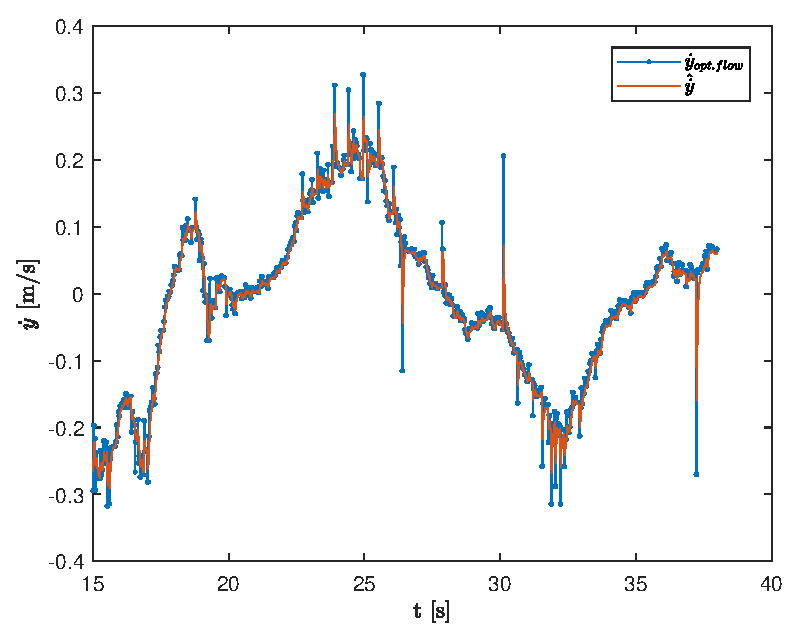
\includegraphics [width=4in]{FlightAnalyzer2_09.eps}


\subsection*{Velocity, Optical Flow}

\begin{verbatim}
eps = 1e-10;
figure('Name','Velocity  & Optical flow');

plot(RSrun_opticalFlow(:,1),1/quadEDT.velocityToOpticalFlow_gain*RSrun_opticalFlow(:,2:3),'-'); hold all;
plot(RSrun_states_estim(:,1),RSrun_states_estim(:,8),'.-');
plot(RSrun_states_estim(:,1),RSrun_states_estim(:,9),'.-');

legend({'$\dot{x}_{opt. flow}$' '$\dot{y}_{opt. flow}$' '$\dot x$' '$\dot y$'},'Interpreter', 'latex','Location','best');
xlabel({'t [s]'},'Interpreter','latex');
ylabel({'[m/s]'},'Interpreter','latex');
%{
%% Battery status
if exist('RSrun_batteryStatus','var')

    figure('Name','Battery voltage');

    plot(RSrun_batteryStatus(:,1),RSrun_batteryStatus(:,3));
    legend('Battery voltage');
    xlabel({'t [s]'},'Interpreter','latex');
    ylabel({'\%'},'Interpreter','latex');
end;
%}
\end{verbatim}

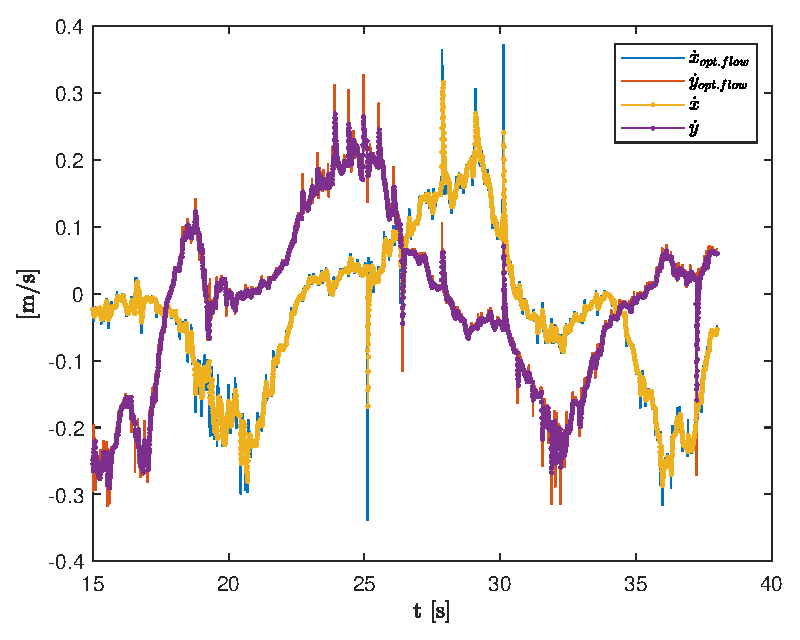
\includegraphics [width=4in]{FlightAnalyzer2_10.eps}



\end{document}
    
